\chapter{CERN, the LHC and LHCb}
\label{CERN_LHC_LHCb}

The European Organisation for Nuclear Research (CERN) was founded in 1954 and began with 12 member states as a organisation to encourage European collaboration and the study of nuclear physics. Since it's foundation the collaborative nature of CERN allowed for large-scale expensive experiments and machines to be built. The Proton Synchrotron was CERN's flagship accelerator, operational in 1959 it had a circumference of 628~m and accelerated protons to 25~\gev, the highest energy at that time. Now 62 years since it's foundation CERN has grown to include 21 member states~\footnote{about the other types of countries involved.} and is still at the forefront of high energy physics research. CERN’s latest accelerator, the Large Hadron Collider (LHC), is most energetic particle accelerator ever built, with a 27~km circumference the LHC was designed to protons at 14~\tev. This chapter shall discuss the LHC and the LHC beauty experiment, one of the experiments that uses collisions provided by the LHC.

\section{The LHC}
\label{LHC}


The LHC is a proton synchrotron that was designed to accelerate and collide two beams of protons travelling in oposite directions up to a center-of-mass energy of 14~\tev. Although operation of the LHC began in 2010 it is yet to reach design energy. The purpose of the LHC is to provide high energy proton collisions, the products of which are used for precision tests of the Standard Model (SM) and to search for new physics particles that go beyond the scope of the SM. There are four interaction points on the LHC ring where the beams are brought to collide, at these points various experiments detect and study the products of these collisions. The LHC can also accelerate lead-nuclei up to an energy of 2.76~\tev per nucleon, but it is only the products from proton collisions that are the topic of this thesis.

%It's the bit below that I'm not a massive fan of the explains how the LHC gets it's protons. I think that it is a little too brief and disconnected with not explanations.
The protons for the LHC originate from hydrogen gas, %add something nice here
the hydrogen atoms are ionised to strip away the electrons and the protons are accelerated through a chain of particle accelerators of increasing energy before being injected into the LHC. The chain of accelerators, shown in Fig.~\ref{fig:accelerator_chain}, consists of existing accelerators that have been used in various experiments through the second half of the last century and have been upgraded to meet the requirements needed to providing protons for the LHC. 
The protons leave the chain of accelerators with of energy of 450~\gev per proton and in bunches of >~$10^{11}$, as the bunches injected into the LHC they are split into two oppositely circulating beams.
The LHC accelerates the protons to the desired center of mass energy using supercooled radio frequency cavities for acceleration and superconducting dipole magnets to bend the beams around the ring. %I could add here some details about the magnets and how the LHC accelerates the protons.
Once the required energy has been reached, the bunches are focused using quadrupole magnets before being brought to collide at 4 interaction point at a bunch crossing rate of 40~MHz. 


\begin{figure}[htbp!] 
  \centering    
  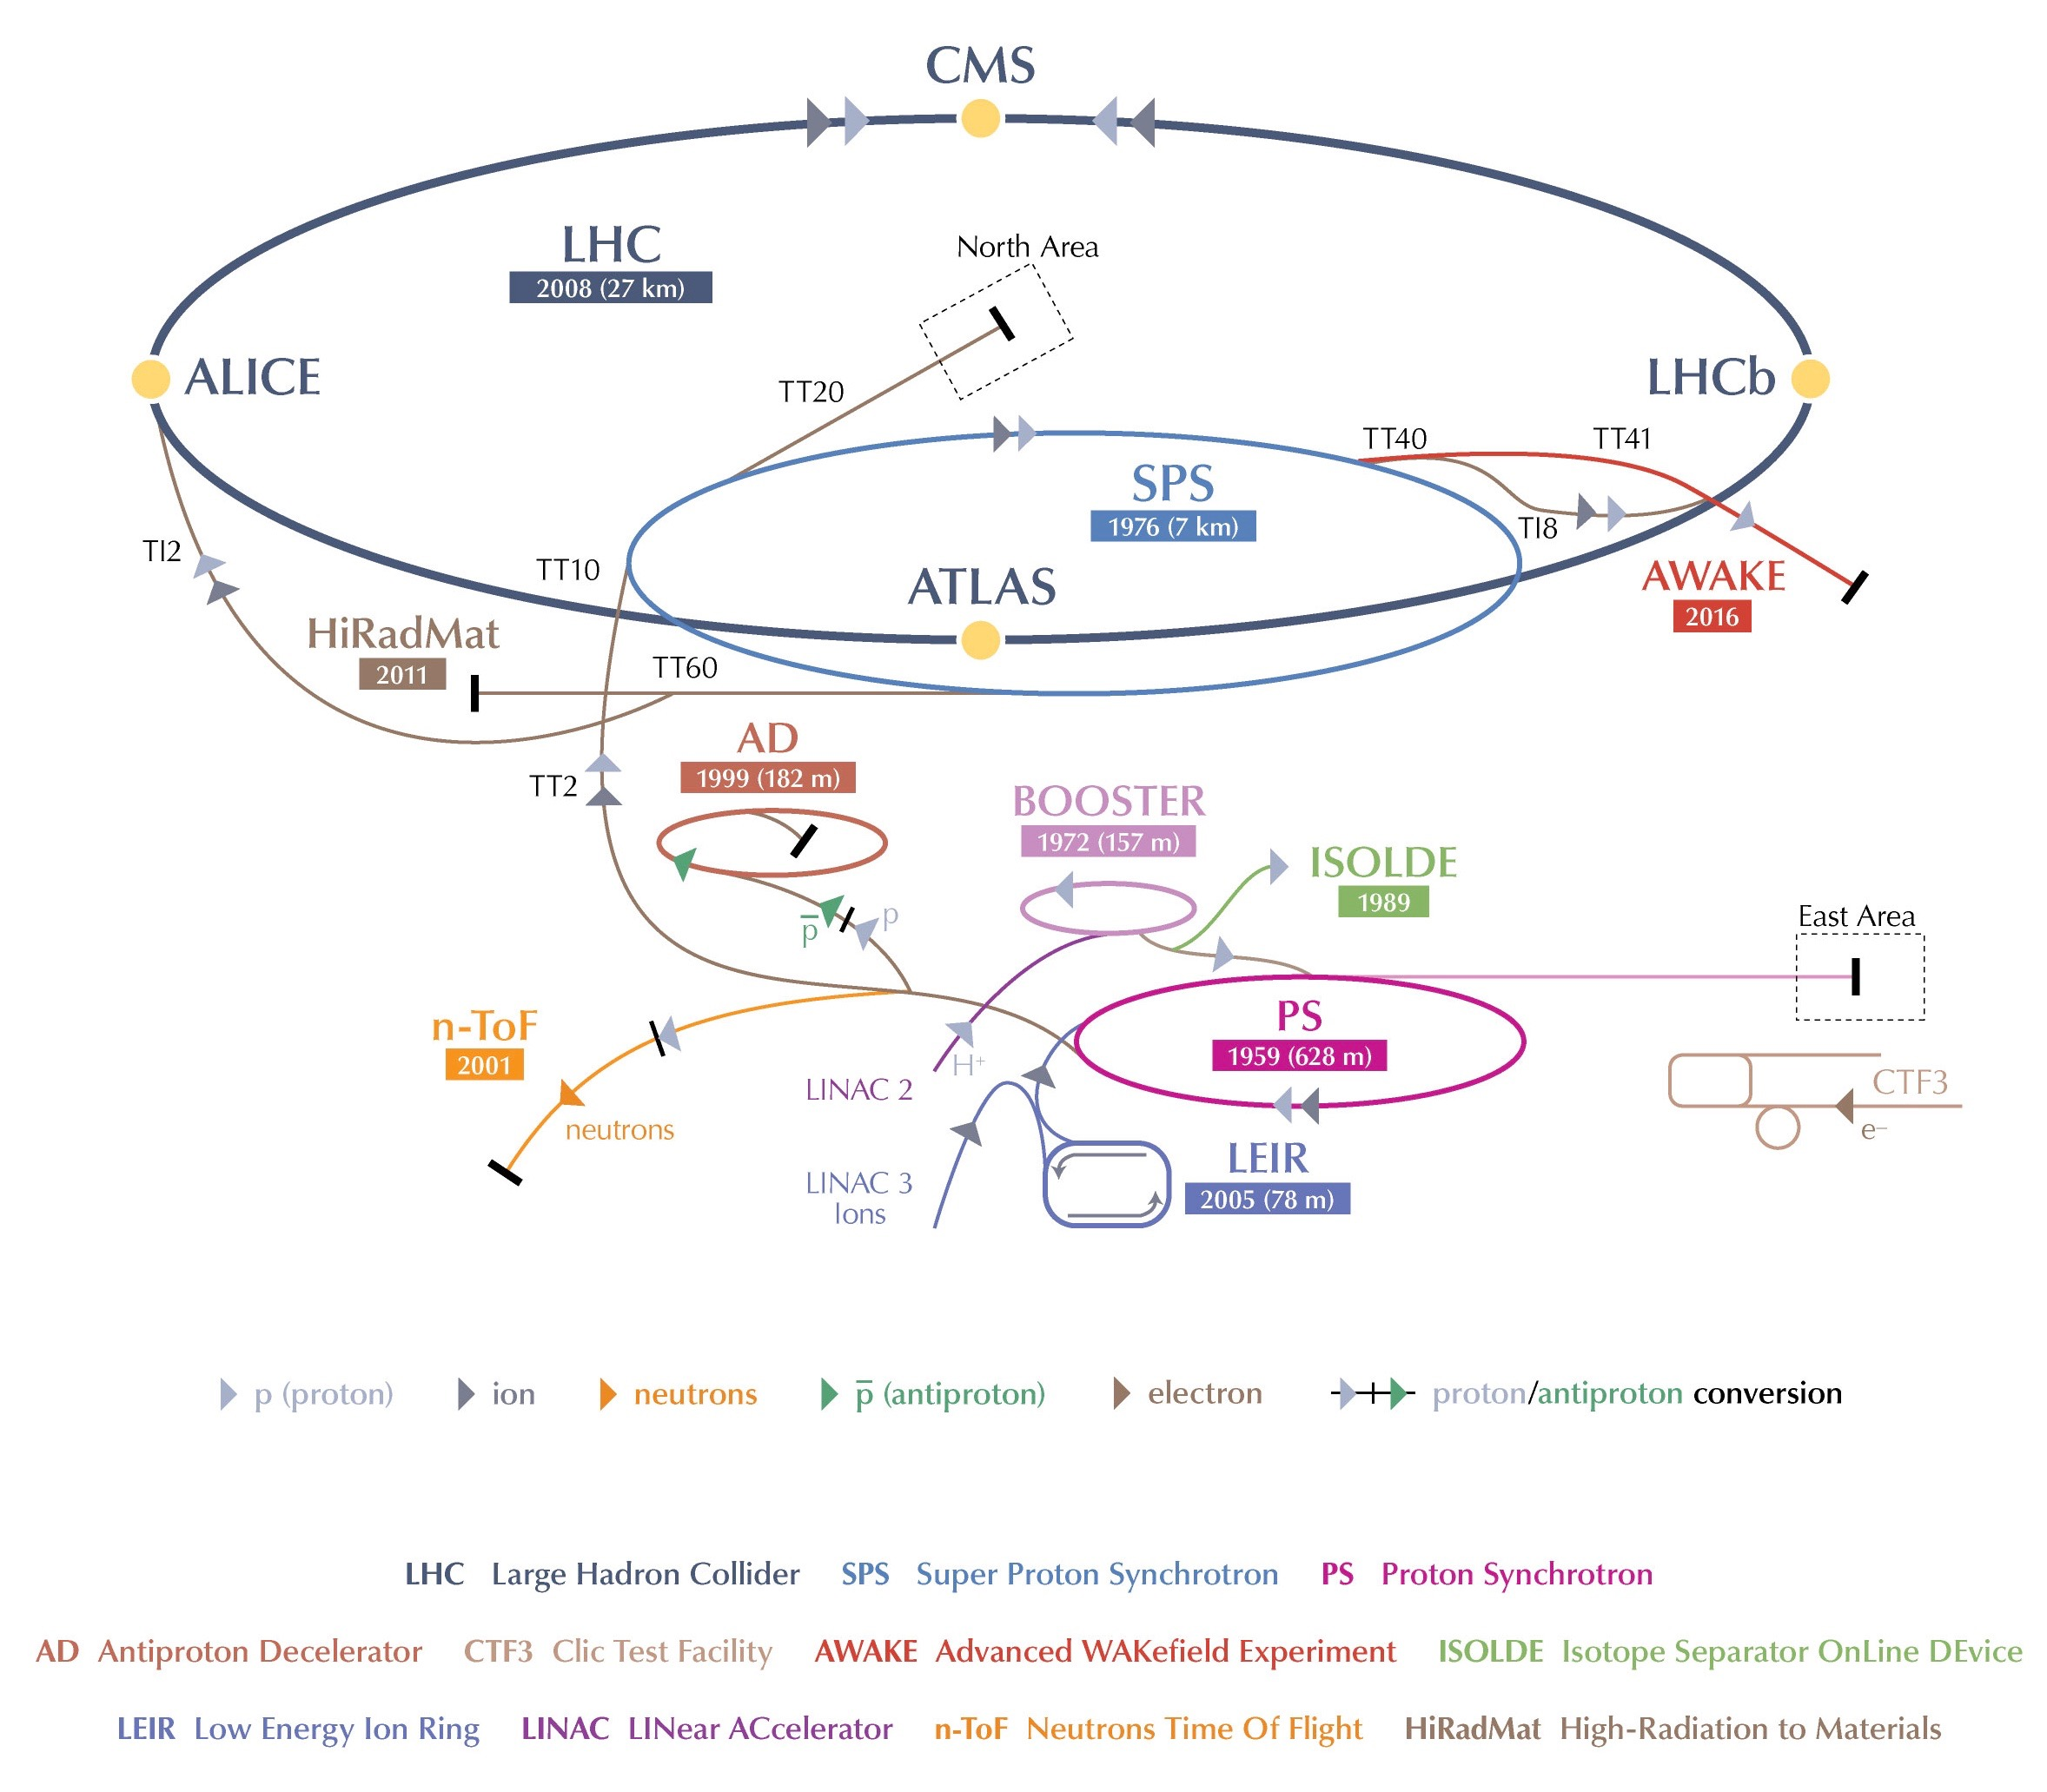
\includegraphics[trim = 125mm 2mm 125mm 90mm, clip, width=1.0\textwidth]{accelerator_complex.jpg}
  \caption{The accelerator complex at CERN. The chain of accelerators used to inject protons into the LHC consists of the Linac 2 accelerating protons to 50~\mev, the Proton Synchrotron Booster accelerating protons to 1.4 \gev, the Proton Synchrotron accelerating protons to 25~\gev and creating the desired spacing between proton bunches then finally the Super Proton Synchrotron accelerating protons to 450~\gev. Source: CERN.}
  \label{fig:accelerator_chain}
\end{figure}




The center of mass energy of a collider is an important measure of it's performance as it dictates what particles can or could be produced in collisions but another important measure of collider performance is the instantaneous luminosity a collider can provide. The instantaneous luminosity, $\mathcal{L}$, is a measure of how many collision occur per second, it is given by

\begin{equation}
\mathcal{L} = \frac{N^{2} f n_{b}}{\mathcal{F}}.
\label{eq:inst_lumi}
\end{equation}


where $N$ is the number of protons per bunch, $n_{b}$ the number of bunches per beam, $f$ the bunch revolution frequency and $\mathcal{F}$ contains information about the beam geometry. The LHC is designed to operate at a maximum instantaneous luminosity of $10^{34}$~cm$^{-2}$s$^{-1}$, in order to reach this luminosity the LHC can have 2808 bunches per beam and a revolution frequency for beams is 11.245 kHz leading to a separation of 25~ns between bunches. The higher the luminosity, the more collisions happen in a second and the more particles will be produced, this can either be advantageous or disadvantageous depending on the physics process that is being studied.
% and the detector design that records the collisions. 
Therefore luminosity delivered at each interaction point can be tuned by the quadrupole magnets by altering the shape of each bunch to suit the experiments at each point.

Proton beams first circulated the LHC in 2008 and since then there have been two physics Runs separated by a long shutdown period. Run 1 began in 2010 and continued until 2013, during this time protons were collided with a center of mass energy of 7~TeV in 2010 and 2011 then this energy was increased to 8~TeV for 2012. After Run~1 came a period in which now collisions occur ed, know as the Long Shutdown~1, during this time work was done to prepare the LHC to operate at higher energies and renovation work was preformed on accelerators that provide the LHC with protons. Run~2 began in 2015 with proton collisions at 13~TeV, %why 13TeV? I have the answer
this Run will continue until 2018 when a second period of upgrades and maintenance, the Long Shutdown~2, will begin.




There are 7 experiments on the LHC that detect particles produced in proton and heavy ion collisions produced during the physics Runs. There are two general purpose detectors, ATLAS and CMS, that were designed to search for the Higgs boson and new particles that are beyond the scope of the SM in proton collisions, these two experiments operate at the full instantaneous luminosity of the LHC. %Perhaps say we found the Higgs?
ALICE studies quark-gluon plasma produced in heavy ions collisions in order to probe conditions similar to those present in the early universe. The TOTEM experiment studies properties of protons as they collide head on at the LHC. The MOEDAL experiment is designed primarily to detect magnetic monopoles, particles carrying magnetic charge which are so far unobserved. The LHCf experiment is a very forward experiment that is designed to detect particles that are thrown forward in LHC collisions which would simulate processes similar to those occurring in cosmic rays. Finally there is the Large Hadron Collider Beauty experiment (LHCb), this experiment was designed to studies rare $b$-hadron decays and $\mathcal{CP}$ violating processes and operates at a lower luminosity that the general purpose detectors. %Should probably include the full experiment names as I have done for LHCb or not include the name for LHCb.




